% coding:utf-8

% Ausführen in R: 
% Sweave("C:/Daten/Daniel/studium/git_repo/sem2/stoc/sw08/sw08_4.Rnw",encoding='UTF-8')

\section{Aufgabe 4}

\subsection{a}
\begin{Schunk}
\begin{Sinput}
> par(mfrow=c(1,2)) # Mehrere Grafiken neben- und untereinander
> werte <- c(0,10,11) # moegliche Werte von X
> sim <- sample(werte,1000, replace = TRUE) # X simulieren
> hist(sim, main=paste("Original")) # Histogramm erstellen
> qqnorm(sim) # Normalplot erstellen
\end{Sinput}
\end{Schunk}
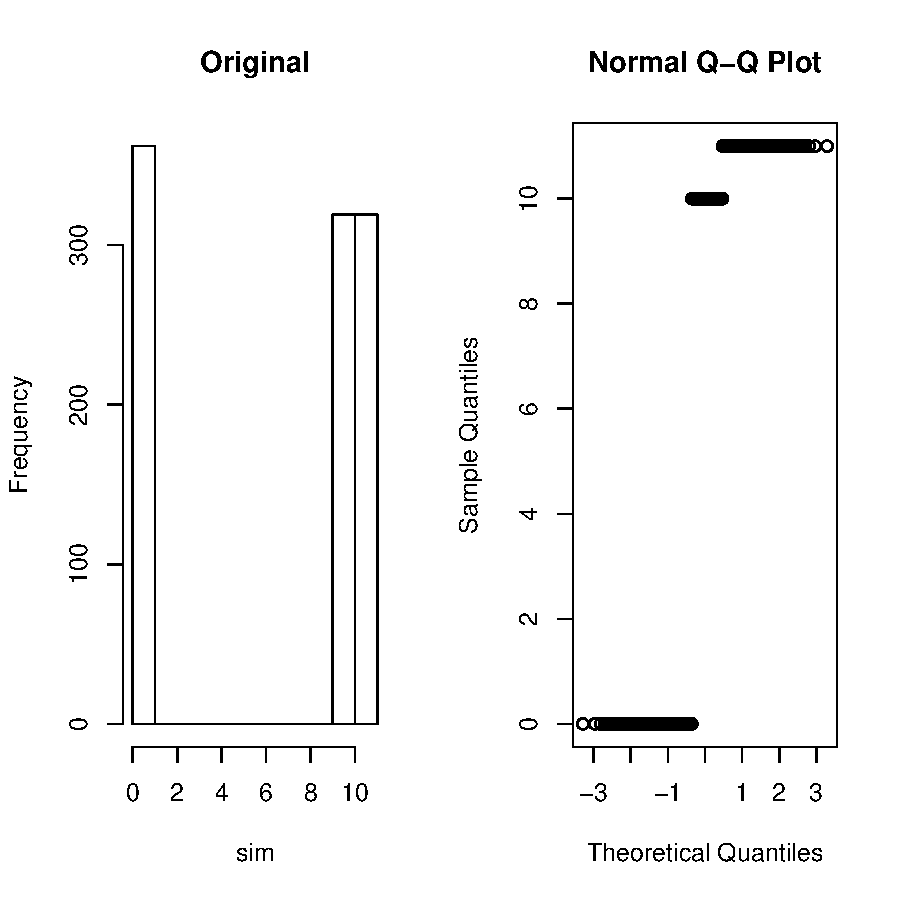
\includegraphics{sw08_4-001}

\subsection{b}
\begin{Schunk}
\begin{Sinput}
> par(mfrow=c(1,2))
> n<-5
> sim<-matrix(sample(werte,n*1000,replace=TRUE),ncol=n)
> # X_1,...,X_n simulieren und in einer n-spaltigen Matrix
> # (mit 1000 Zeilen) anordnen
> sim.mean<- apply(sim,1,"mean") #In jeder Matrixzeile Mittelwert berechnen
> hist(sim.mean)
> title(paste("Mittelwerte von",n,"Beobachtungen"))
> qqnorm(sim.mean)
\end{Sinput}
\end{Schunk}
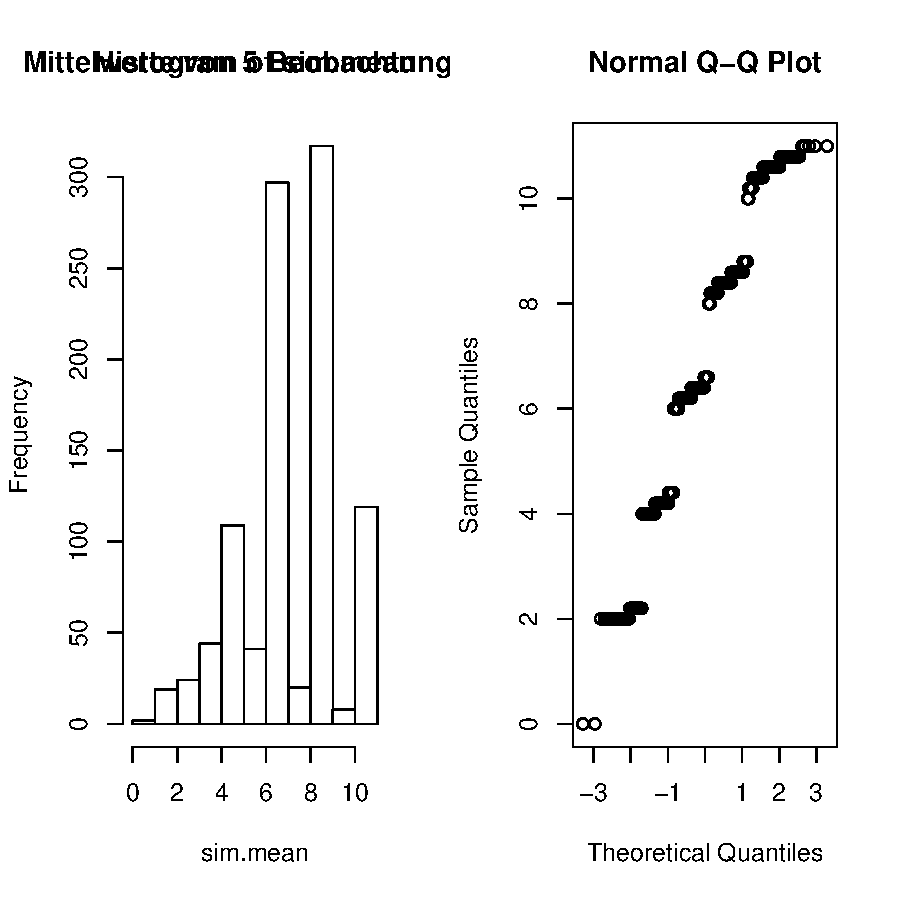
\includegraphics{sw08_4-002}

\subsection{c}
\begin{Schunk}
\begin{Sinput}
> par(mfrow=c(1,2))
> n<-5
> sim<-matrix(sample(werte,n*10,replace=TRUE),ncol=n)
> # X_1,...,X_n simulieren und in einer n-spaltigen Matrix
> # (mit 10 Zeilen) anordnen
> sim.mean<- apply(sim,1,"mean") #In jeder Matrixzeile Mittelwert berechnen
> hist(sim.mean)
> title(paste("Mittelwerte von",n,"Beobachtungen"))
> qqnorm(sim.mean)
\end{Sinput}
\end{Schunk}
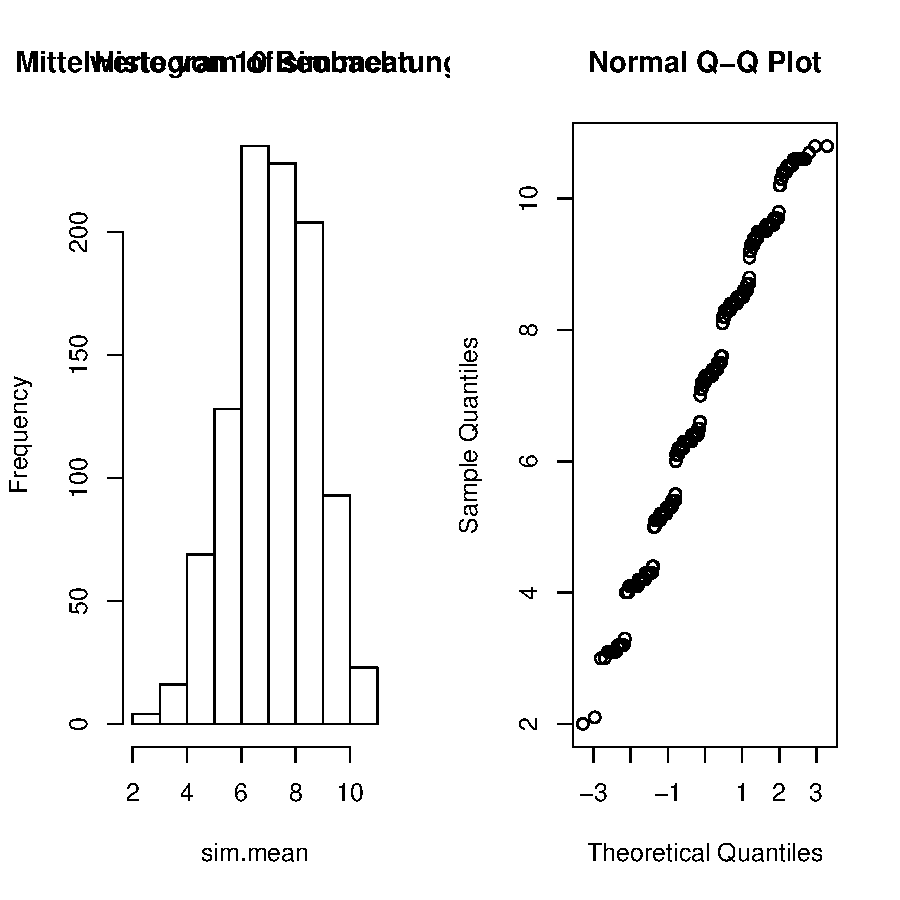
\includegraphics{sw08_4-003}

\begin{Schunk}
\begin{Sinput}
> par(mfrow=c(1,2))
> n<-5
> sim<-matrix(sample(werte,n*200,replace=TRUE),ncol=n)
> # X_1,...,X_n simulieren und in einer n-spaltigen Matrix
> # (mit 200 Zeilen) anordnen
> sim.mean<- apply(sim,1,"mean") #In jeder Matrixzeile Mittelwert berechnen
> hist(sim.mean)
> title(paste("Mittelwerte von",n,"Beobachtungen"))
> qqnorm(sim.mean)
\end{Sinput}
\end{Schunk}
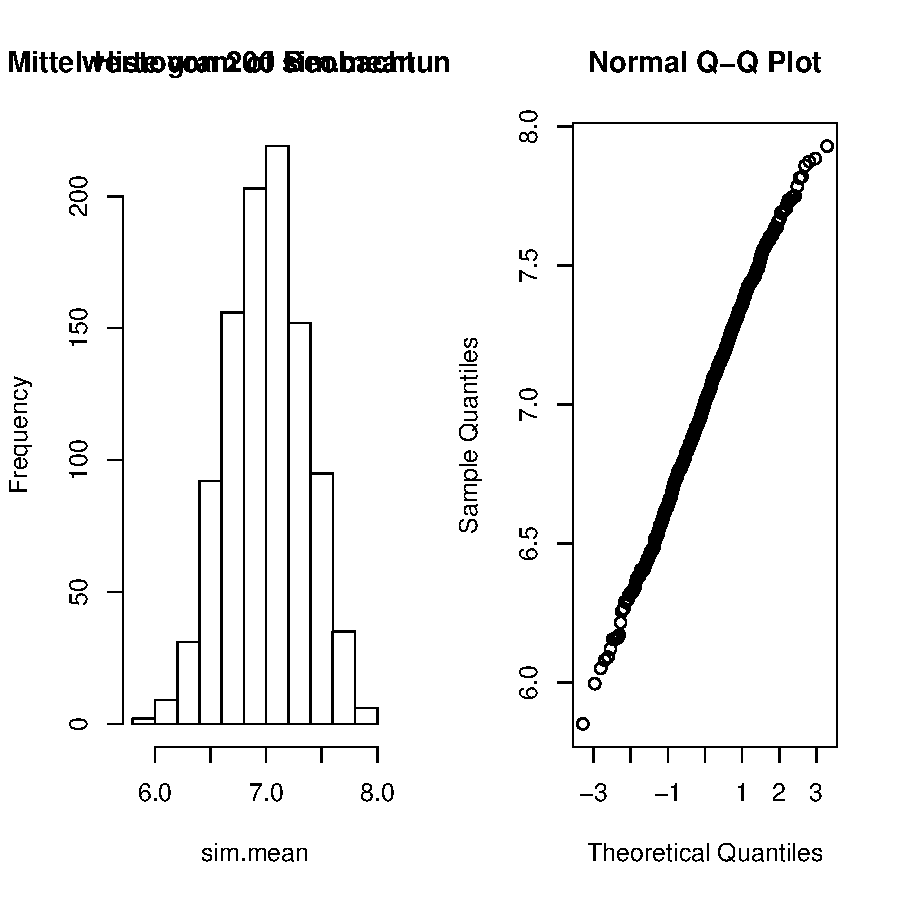
\includegraphics{sw08_4-004}

